\documentclass[10pt,a4paper, margin=1in]{article}
\usepackage{fullpage}
\usepackage{amsfonts, amsmath, pifont}
\usepackage{amsthm}
\usepackage{graphicx}

\usepackage{tkz-euclide}
\usepackage{tikz}
\usepackage{pgfplots}
\pgfplotsset{compat=1.13}

\usepackage{geometry}
 \geometry{
 a4paper,
 total={210mm,297mm},
 left=10mm,
 right=10mm,
 top=10mm,
 bottom=10mm,
 }
 
\begin{filecontents}{q3a.dat}
 n   xn
 4 1
 3 0
 2 0
 1  3
 0   2
 -1   0  
 -2   0
 -3   6
 -4   0
\end{filecontents}

\begin{filecontents}{q3b.dat}
 n   xn
 -4 0
 -3 0
 -2 1
 -1  1
 0  0
 1   -1  
 2   -1
 3   0
 4   0
\end{filecontents}


\begin{filecontents}{q2b.dat}
 n   xn
 0  0
 1   1
 2   -1
 3   1
 4   -1
\end{filecontents}
 
 % Write both of your names here. Fill exxxxxxx with your ceng mail address.
 \author{
  Uçan, Yiğitcan\\
  \texttt{e2310555@ceng.metu.edu.tr}
  \and
  Akın, Ozan\\
  \texttt{e2309599@ceng.metu.edu.tr}
}
\title{CENG 384 - Signals and Systems for Computer Engineers \\
Spring 2021 \\
Homework 2}
\begin{document}
\maketitle



\noindent\rule{19cm}{1.2pt}

\begin{enumerate}

\item %write the solution of q1
    \begin{enumerate}
    % Write your solutions in the following items.
    \item %write the solution of q1a
    \[ x(t) + -5y(t) - 6  \int_{\tau=-\infty}^{} y(\tau) \,d\tau = \dot{y}(t)\]
    \[ \dot{x}(t) - 5\dot{y}(t) - 6y(t) = \ddot{y}(t)\]
    \[ \ddot{y}(t) + 5\dot{y}(t) + 6y(t) = \dot{x}(t)\]
    \item %write the solution of q1b
    \[ y_h(t) = C_1e^{-5t} + C_2e^{-t} \]
    \[ y_p(t) = K(e^{-t} + e^{-4t}) u(t) \]
    \[ \dot{y}_p(t) = K(-e^{-t} -4e^{-4t}) u(t) \]
    \[ \ddot{y}_p(t) = K(e^{-t} + 16 e^{-4t}) u(t) \]
    \[ K(e^{-t} + 16 e^{-4t}) + 5K(-e^{-t} -4e^{-4t}) + 6K(e^{-t} + e^{-4t}) = (e^{-t} + e^{-4t}) \]
    \[ 2K(e^{-t} + e^{-4t}) = (e^{-t} + e^{-4t}) \]
    \[ K = \frac{1}{2} \]
    \[ y_p(t) = K x(t) = \frac{e^{-t} + e^{-4t}}{2} u(t) \]
    \[ y(t) = y_h(t) + y_p(t) = C_1e^{-5t} + C_2e^{-t} + \frac{e^{-t} + e^{-4t}}{2} u(t) \]
    \[ \dot{y}(t) = -5C_1e^{-5t} - C_2e^{-t} - \frac{e^{-t} + 4e^{-4t}}{2} \cdot u(t) \]
    \[ y(0) = 0 , \dot{y}(0) = 0 \]
    \[ y(0) = C_1 + C_2 + 1 \]
    \[ \dot{y}(0) = -5C_1 - C_2 - \frac{5}{2} = 0 \]
    \[ C_1 = \frac{-3}{8}, C_2 = \frac{-5}{8} \]
    \[ y(t) = \frac{-3}{8} e^{-5t} + \frac{-5}{8} e^{-t} + \frac{e^{-t} + e^{-4t}}{2} u(t) \]
    \end{enumerate}

\item %write the solution of q2
    \begin{enumerate}
    % Write your solutions in the following items.
    \item %write the solution of q2a
    \[ x_1[n] = x[n] - x[n-2] \] \\ 
    With the time invariance property $x[n-2] \Rightarrow y[n-2] = \delta[n-3]$. \\
    With the superposition property $-x[n-2] \Rightarrow -y[n-2] = -\delta[n-3]$. \\
    \[ x_1[n] = x[n] - x[n-2] \Rightarrow y_1[n] = y[n] - y[n-2] = \delta[n-1] - \delta[n-3]\]
    \item %write the solution of q2b
\[ y[n] = x[n] * h[n] \]
\[ y[n] = \sum_{k=-\infty}^{\infty} x[n-k] \cdot h[k] \]
\[ \delta[n-1] = \sum_{k=-\infty}^{\infty} (\delta[n-k] + \delta[n-1-k]) \cdot h[k] \]
\[ \delta[n-1] = h[n] + h[n-1] \]
\[ h[n] = \delta[n-1] - h[n-1] \]  

\[ h[0] = 0 \]
\[ h[1] = \delta[0] - h[0] = 1 \]
\[ h[2] = \delta[1] - h[1] = -1\]
\[ h[3] = \delta[2] - h[2] = 1\]
\[ h[n] = (-1)^{n} u[n-1]\]

\begin{figure} [h!]
    \centering
    \begin{tikzpicture}[scale=1.0] 
      \begin{axis}[
          axis lines=middle,
          xlabel={$n$},
          ylabel={$\boldsymbol{h[n]}$},
          xtick={-1, -3, -2, -1, ..., 4},
          ytick={-3, -2, -1, ..., 3},
          ymin=-3, ymax=3,
          xmin=-1, xmax=4,
          every axis x label/.style={at={(ticklabel* cs:1.05)}, anchor=west,},
          every axis y label/.style={at={(ticklabel* cs:1.05)}, anchor=south,},
          grid,
        ]
        \addplot [ycomb, black, thick, mark=*] table [x={n}, y={xn}] {q2b.dat};
      \end{axis}
    \end{tikzpicture}
    \caption{$h[n]$ - q2b}
    \label{fig:q3}
\end{figure}

    \item %write the solution of q2c 
    
\[ y[n] = x[n-1] - y[n-1]\]
    \item %write the solution of q2d
~\\
\begin{center}
	\tikzset{%
		block/.style    = {draw, thick, rectangle, minimum height = 3em,
			minimum width = 3em},
		sum/.style      = {draw, circle, node distance = 2cm}, % Adder
		input/.style    = {coordinate}, % Input
		output/.style   = {coordinate} % Output
	}
	% Defining string as labels of certain blocks.
	\newcommand{\suma}{\Large$+$}
	\newcommand{\inte}{$\displaystyle \int$}
	\newcommand{\derv}{\huge$\frac{d}{dt}$}
	
	\begin{tikzpicture}[auto, thick, node distance=2cm, >=triangle 45]
	\draw
	% Drawing the blocks of first filter :
	node at (0, 0) [input] (inp) {\Large \textopenbullet}
	node [block, right of=inp] (inp2) {$D$}
	node [sum, right of=inp2] (sum) {\suma}
	node [output, right of=sum] (out) {}
	node [block, below of=out] (dec) {$D$}
	node [output, right of=out] (out2) {\Large \textopenbullet}
	node [output, below of=sum] (temp) {}
	;
	\draw[->](inp) -- node{$x[n]$} (inp2);
	\draw[->](inp2) -- (sum);
	\draw[-](sum) -- (out);
	\draw[->](out) -- node{$y[n]$} (out2);
	\draw[->](out) -- (dec);
	\draw[-](dec) -- node{$-$} (temp);
	\draw[->](temp) -- (sum);
	\end{tikzpicture}
\end{center}

    \end{enumerate}

\item %write the solution of q3  
    \begin{enumerate}
    % Write your solutions in the following items.
    \item %write the solution of q3a
    $\delta[0] \cdot \delta[n] = \delta[n]$
    \[ \sum_{k=-\infty}^{\infty} (\delta[k-3] + 2\delta[k+1])(\delta[n-k-1] + 3\delta[n-k+2]) \]
    \[ = (\delta[n-4] + 3\delta[n-1]) + 2(\delta[n] + 3\delta[n+3])\]
    \[ = 6\delta[n+3] + 2\delta[n] + 3\delta[n-1] + \delta[n-4]  \]
    
\begin{figure} [h!]
    \centering
    \begin{tikzpicture}[scale=1.0] 
      \begin{axis}[
          axis lines=middle,
          xlabel={$n$},
          ylabel={$\boldsymbol{y[n]}$},
          xtick={-4, -3, -2, -1, ..., 4},
          ytick={-6, -5, -4, ..., 6},
          ymin=-6, ymax=6,
          xmin=-4, xmax=4,
          every axis x label/.style={at={(ticklabel* cs:1.05)}, anchor=west,},
          every axis y label/.style={at={(ticklabel* cs:1.05)}, anchor=south,},
          grid,
        ]
        \addplot [ycomb, black, thick, mark=*] table [x={n}, y={xn}] {q3a.dat};
      \end{axis}
    \end{tikzpicture}
    \caption{$y[n]$ - q3a}
    \label{fig:q3}
\end{figure}

    \item %write the solution of q3b
    $u[0] \cdot u[n] = u[n]$
    \[ \sum_{k=-\infty}^{\infty} (u[k+3] - u[k])(u[n-k-1] - u[n-k-3]) \]
    \[ = (u[n+2] - u[n]) - (u[n-1] - u[n-3])\]
    \[ = u[n+2] - u[n] - u[n-1] + u[n-3]  \]
    
    
\begin{figure} [h!]
    \centering
    \begin{tikzpicture}[scale=1.0] 
      \begin{axis}[
          axis lines=middle,
          xlabel={$n$},
          ylabel={$\boldsymbol{y[n]}$},
          xtick={-4, -3, -2, -1, ..., 4},
          ytick={-6, -5, -4, ..., 6},
          ymin=-6, ymax=6,
          xmin=-4, xmax=4,
          every axis x label/.style={at={(ticklabel* cs:1.05)}, anchor=west,},
          every axis y label/.style={at={(ticklabel* cs:1.05)}, anchor=south,},
          grid,
        ]
        \addplot [ycomb, black, thick, mark=*] table [x={n}, y={xn}] {q3b.dat};
      \end{axis}
    \end{tikzpicture}
    \caption{$y[n]$ - q3b}
    \label{fig:q3}
\end{figure}
    
    %write the solution of q6b
    \end{enumerate}

\newpage 

\item %write the solution of q4
    \begin{enumerate}
    % Write your solutions in the following items.
    \item %write the solution of q4a
    \[ \int_{\tau=-\infty}^{\infty} e^{-3(t-\tau)} u(t - \tau) \cdot e^{-2\tau} u(\tau) \,d\tau \]
    \[ e^{-3t} \int_{\tau=0}^{t} e^{3\tau} \cdot e^{-2\tau} \,d\tau \]
    \[ e^{-3t} \int_{\tau=0}^{t} e^{\tau} \,d\tau \]
    \[ e^{-3t} \cdot (e^{t} - 1) = e^{-2t} - e^{-3t} \]
    \item %write the solution of q4b
    \[ \int_{\tau=-\infty}^{\infty} e^{2(t-\tau)} u(t - \tau) \cdot (u(\tau) - u(\tau - 2)) \,d\tau \]
    \[ e^{2t} \cdot \int_{\tau=-\infty}^{\infty} e^{-2\tau} u(t - \tau) u(\tau) - e^{-2\tau} u(t - \tau) u(\tau - 2) \,d\tau \]
    \[ e^{2t} \cdot (\int_{\tau=0}^{t} e^{-2\tau} \,d\tau - \int_{\tau=2}^{t} e^{-2\tau} \,d\tau) \]
    \[ e^{2t} \cdot (\frac{1 - e^{-2t}}{2} - \frac{e^{-4} - e^{-2t}}{2}) \]
    \[\frac{e^{2t} - 1}{2} - \frac{e^{2t - 4} - 1}{2} \]
    \[\frac{e^{2t} - e^{2t-4}}{2} \]
    \end{enumerate}

\item %write the solution of q5
    \begin{enumerate}
    % Write your solutions in the following items.
    \item %write the solution of q5a

\[ h[n] = s[n] - s[n-1] = n \cdot u[n] - (n-1) \cdot u[n-1]  = u[n] \cdot(n - (n-1))\]
\[ h[n] = u[n] \]
    \item %write the solution of q5b
\[ y[n] = x[n] * h[n] \]
\[ x[n] = h^{-1}[n] * y[n] \]
\[ h[n] * h^{-1}[n] = \delta[n] \]
\[ \sum_{k=-\infty}^{\infty} h[n - k] \cdot h^{-1}[k] = \delta[n] \]
\[ \sum_{k=-\infty}^{\infty} u[n - k] \cdot \delta[k] = \delta[n] \]
\[ h^{-1}[n] = \delta[n] - \delta[n-1] \]
\[ x[n] = \sum_{k=-\infty}^{\infty} y[n - k] \cdot h^{-1}[k] \]
\[ x[n] = \sum_{k=-\infty}^{\infty} (\delta[n-k] - \delta[n-1-k]) \cdot (\delta[k] - \delta[k-1]) \]
\[ x[n] = \delta[n] - \delta[n-1] - \delta[n-1] + \delta[n-2] \]

    \item %write the solution of q5c
    
\[ x[n] = \delta[n] - \delta[n-1] - \delta[n-1] + \delta[n-2] \]
\[ y[n] = \delta[n] - \delta[n-1] \]
\[ y[n-1] = \delta[n-1] - \delta[n-2] \]
\[ -y[n-1] = -\delta[n-1] + \delta[n-2] \]
\[ x[n] = y[n] - y[n-1]\]
    \end{enumerate}

\item %write the solution of q6

\[ h(t) = \frac{ds(t)}{dt} = t \cdot u(t) \]

\[ y(t) = x(t) * h(t) \]

\[ y(t) = \int_{\tau=-\infty}^{\infty} x(t - \tau) \cdot h(\tau) \,d\tau \]

\[ y(t) = \int_{\tau=-\infty}^{\infty} (e^{-(t-\tau)} \cdot u(t - \tau)) \cdot (\tau \cdot u(\tau)) \,d\tau \]

\[ y(t) = e^{-t} \int_{\tau=0}^{t} e^{\tau} \cdot \tau \,d\tau \]

\[ y(t) = e^{-t} \cdot (e^{t} \cdot (t - 1) + 1) \]

\[ y(t) = t - 1 + e^{-t} \]

\item %write the solution of q7
    \begin{enumerate}
    % Write your solutions in the following items.
    \item %write the solution of q7a
    \[ h(t) = u(t) \cdot (\delta(t-3) -\delta(t-5)) = u(t-3) - u(t-5) \]
    
    \begin{figure}[h!]
    \centering
        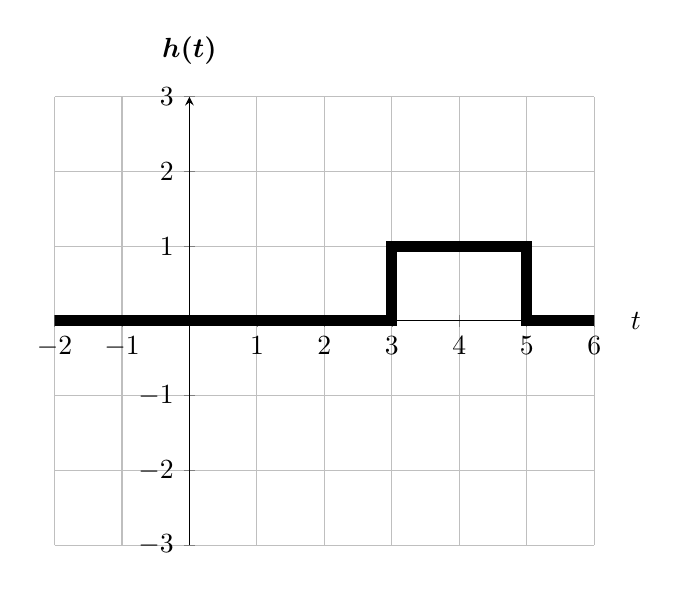
\begin{tikzpicture}[scale=1.0]
           \begin{axis}[
          axis lines=middle,
          xlabel={$t$},
          ylabel={$\boldsymbol{h(t)}$},
          xtick={-2, -1, 0, 1, ..., 6},
          ytick={-3, -2, -1, ..., 3},
          ymin=-3, ymax=3,
          xmin=-2, xmax=6,
          every axis x label/.style={at={(ticklabel* cs:1.05)}, anchor=west,},
          every axis y label/.style={at={(ticklabel* cs:1.05)}, anchor=south,},
          grid,
        ]
           \path[draw,line width=4pt] (-4,0) -- (3,0) -- (3,1) -- (5,1) -- (5,0) -- (6,0);
           \end{axis}
        \end{tikzpicture}
        \caption{Impulse response of the system}
        \label{fig:q2}
    \end{figure}
    
    \newpage
    
    \item %write the solution of q7b
    \[ y(t) = x(t) * h(t) \]
    \[ y(t) = \int_{\tau=-\infty}^{\infty} e^{-3(t-\tau)} u(t - \tau) \cdot (\delta(\tau-3) - \delta(\tau-5)) u(\tau) \,d\tau \]
    \[ y(t) = \int_{\tau=-\infty}^{\infty} e^{-3(t-\tau)} u(t - \tau) \cdot u(\tau-3)  \,d\tau - \int_{\tau=-\infty}^{\infty} e^{-3(t-\tau)} u(t - \tau) \cdot u(\tau-5) \,d\tau \]
    \[ y(t) = \int_{\tau=3}^{t} e^{-3(t-\tau)} \,d\tau - \int_{\tau=5}^{t} e^{-3(t-\tau)} \,d\tau \]
    \[ y(t) = e^{-3t} (\int_{\tau=3}^{t} e^{3\tau} \,d\tau - \int_{\tau=5}^{t} e^{3\tau} \,d\tau) \]
    \[ y(t) = e^{-3t} (\frac{e^{3t} - e^9}{3} - \frac{e^{3t} - e^{15}}{3}) \]
    \[ y(t) = e^{-3t} \frac{e^{15} - e^9}{3} \]
    \item %write the solution of q7c
    \[ \frac{dh(t)}{d(t)} = \delta(t-3) - \delta(t-5)\]
    
    
    \[ g(t) = \int_{\tau=-\infty}^{\infty} (\delta(\tau-3) - \delta(\tau-5)) \cdot e^{-3(t-\tau)} u(t-\tau)  \,d\tau \]
    \[ g(t) = \int_{\tau=-\infty}^{\infty} (\delta(\tau-3) - \delta(\tau-5)) \cdot e^{-3(t-\tau)} u(t-\tau)  \,d\tau \]
    \[ g(t) = e^{-3t} (\int_{\tau=-\infty}^{t} \delta(\tau-3) \cdot e^{3\tau}  \,d\tau - \int_{\tau=-\infty}^{t} \delta(\tau-5) \cdot e^{3\tau}  \,d\tau ) \]
    \[ g(t) = e^{-3t} (e^9 \cdot (u(t-3) - u(t-5))) \]
    \[ g(t) = e^{-27t} (u(t-3) - u(t-5)) \]
    
    % \[ g(t) = \int_{\tau=-\infty}^{\infty} (\delta(t-3-\tau) - \delta(t-5-\tau)) \cdot e^{-3(\tau)} u(\tau)  \,d\tau \]
    % \[ g(t) = \int_{\tau=-\infty}^{\infty} u(t-3-\tau) \cdot e^{-3(\tau)} \,d\tau - \int_{\tau=-\infty}^{\infty} u(t-5-\tau) \cdot e^{-3(\tau)}  \,d\tau \]
    % \[ g(t) = \int_{\tau=-\infty}^{t-3} e^{-3(\tau)} \,d\tau - \int_{\tau=-\infty}^{t-5} e^{-3(\tau)} \,d\tau \]
    \end{enumerate}    

\end{enumerate}
\end{document}


